\documentclass[a4paper,12pt]{article}

% Import the deliverable package from common directory
\usepackage{../common/deliverable}

% Tell LaTeX where to find graphics files
\graphicspath{{../common/logos/}{./figures/}{../}}

\usepackage{xspace}
\usepackage{lipsum}
\usepackage{booktabs}

% Set the deliverable number (without the D prefix, it's added automatically)
\setdeliverableNumber{2.3}

% Begin document
\begin{document}

% Create the title page with the title as argument
\maketitlepage{Report on application improvements - III semester}

\newpage

% Main Table using the new environment and command
\begin{deliverableTable}
    \tableEntry{Deliverable title}{Report on application improvements - III semester}
    \tableEntry{Deliverable number}{D2.3}
    \tableEntry{Deliverable version}{v1}
    \tableEntry{Date of delivery}{February 28, 2026}
    \tableEntry{Actual date of delivery}{February 28, 2026}
    \tableEntry{Nature of deliverable}{Report}
    \tableEntry{Dissemination level}{Public}
    \tableEntry{Work Package}{WP2}
    \tableEntry{Partner responsible}{FAU}
\end{deliverableTable}

% Abstract and Keywords Section
\begin{deliverableTable}
    \tableEntry{Abstract}{We report on the progress in the biomedical applications that leverage the high-performance and exascale computing capabilities of deal.II. These include lung modeling (TUM), cardiac modeling (POLIMI), brain modeling (FAU), liver modeling (WIAS), and cell mechanobiology (UNIBS). Additionally, we report on the advancements of the low-code/no-code interface developed by Dualistic/eXact-Lab.}
    \tableEntry{Keywords}{Applications; Exascale; Lung; Heart; Brain; Liver; Cell}
\end{deliverableTable}

\newpage

\begin{documentControl}
    \addVersion{0.1}{13/02/2026}{Alexander Greiner (FAU)}{Initial draft with info of all partners}
    \addVersion{0.2}{25/02/2026}{Alexander Greiner (FAU)}{Collection of input from all partners}
    \addVersion{0.3}{28/02/2026}{Martin Kronbichler}{Minor improvements}
    \addVersion{1.0}{28/02/2026}{Alexander Greiner}{Final version}
\end{documentControl}

\subsection*{{Approval Details}}
Approved by: Martin Kronbichler \\
Approval Date: February 28, 2026

\subsection*{{Distribution List}}
\begin{itemize}
    \item [] - Project Coordinators (PCs)
    \item [] - Work Package Leaders (WPLs)
    \item [] - Steering Committee (SC)
    \item [] - European Commission (EC)
\end{itemize}

\vspace*{2cm}

\disclaimer

\newpage

\tableofcontents % Automatically generated and hyperlinked Table of Contents

\newpage

\section{{Introduction}}

In this document, we report on the status of the exascale human applications part of the dealii-X project:
\begin{itemize}
    \item Lungs (TUM)
    \item Heart (POLIMI)
    \item Brain (FAU)
    \item Liver (FVB-WIAS)
    \item Mechanobiology (UNIBS)
\end{itemize}
Additionally, we report on the advancements of the low-code/no-code interface developed by Dualistic/eXact-Lab.

\subsection{{Purpose of the Document}}

This report collects the updates from the project partners (TUM, POLIMI, FAU, FVB-WIAS, UNIBS, Dualistic/eXact-Lab) into a single document. Each section reports on advancements on the corresponding application, and identifies the upcoming steps in the project.

\subsection{{Structure of the Document}}
\begin{itemize}
    \item Section \ref{sec:section2}: Reports on Applications
\end{itemize}

\newpage

\section{{Reports on applications}}
\label{sec:section2}

\subsection{Lungs (TUM)}

This section reports on the progress of the lung application. As mentioned in the outlook section of Deliverable D2.2, this semester, we have mainly been working on implementing the surfactant formulation in the structural module of ExaDG.

The surfactant model is based on an enhanced-surface finite element formulation. This formulation does not directly resolve the fluid lining of the alveoli or the surfactant molecules, but rather indirectly incorporates the nonlinear, time- and frequency-dependent mechanics of surface tension at the element boundary. The resulting weak form contains an additional boundary integral of the surface tension as a multivariate function of the current solution and the local history data of the surfactant model.

Although the ExaDG software had been designed to be easily extensible along several directions, we found that the required implementation of the surfactant formulation did not comply with several key assumptions in the structural module, specifically the material interface and the assumption that boundary terms are independent of the solution. Hence, the implementation required major changes in the boundary integral evaluation routines. Substantial progress was made in this regard, and we are now at a promising stage of the implementation, with the most critical issues resolved. Thus, we expect to finalize this work in the first half of March 2026.

In parallel, we have made initial progress in conducting simulations on the alveolar geometry with basic surface tension effects included. However, this proved more challenging than anticipated, and we have not yet been able to obtain converged results for arbitrary problem setups. This may be because any imperfections in the complex boundary of the alveolar geometry would have an amplified effect on convergence when the problem is driven by surface tension. We are currently investigating this issue, and resolving it will allow us to advance the performance and scalability aspects of our application and integrate new functionality currently developed in the groups of WP1.


% \begin{figure}
%   \centering
%   \includegraphics[width=0.45\textwidth]{xxx.png}
%   \caption{xxx.}
%   \label{fig:xxx}
% \end{figure}

\subsection{Heart (POLIMI)}

This section reports on recent updates to the cardiac modeling library lifex, which relies on deal.II to provide a comprehensive multiphysics framework for simulating the cardiac function.

As mentioned in Deliverable D2.2, we continued the migration of the lifex library toward matrix-free algorithms and the substitution of the \texttt{dealii::FEValues} class with the \texttt{dealii::FEEvaluation} class to improve the performance of matrix-based algorithms.

We implemented the solver for cardiac mechanics and compared the scalability of the previous matrix-based implementation of the solver with the new matrix-based and the matrix-free versions (Figure \ref{fig:lifex_scalability}). The code was tested on structured hexahedral meshes of a beam, with the number of degrees of freedom on the order of millions, while varying the polynomial degree. We observe a slight reduction in computational time when replacing \texttt{dealii::FEValues} class with \texttt{dealii::FEEvaluation} class in the matrix-based approach. As the polynomial degree increases, the matrix-based approaches exhibit a loss of strong scalability due to the lower sparsity of the stiffness matrix and the corresponding increased number of communications between processors, whereas the matrix-free algorithm preserves strong scalability. For low polynomial degrees (1 or 2), the matrix-free approach results in computational times that are higher than or comparable to those of the matrix-based methods. However, for polynomial degree 2 and a large number of parallel processes, the matrix-free implementation achieves lower computational times than the matrix-based ones, owing to its superior strong scalability.

\begin{figure}[h]
  \centering
  
\includegraphics[width=\textwidth]{figures/POLIMI/figure_1.png}
  \caption{Strong scalability of the lifex mechanics solver, in the previous (matrix-based) implementation and new (matrix-based and matrix-free) implementation.}
  \label{fig:lifex_scalability}
\end{figure}

To precondition the linear system arising from cardiac mechanics, we employed the \texttt{dealii::PreconditionChebyshev} class. We also implemented support for the p-multigrid method within the matrix-free framework, which we plan to test for high degree polynomials \citep{schussnig2025matrixfree}.

Based on the progress of the perfusion solver in Deliverable D2.2, we have developed a \emph{Porosolver} that integrates multicompartment Darcy perfusion physics with cardiac mechanics. The framework also includes a module for the generation of rule-based cardiac fiber architectures following the methodology proposed by \citet{piersanti2021modeling}.
The resulting \emph{Porosolver} features a modular architecture and supports three operating modes:
\begin{itemize}
    \item Standalone solid mechanics simulations,
    \item Standalone multicompartment perfusion simulations,
    \item Fully coupled poromechanics simulations within a porous media formulation.
\end{itemize}
For the coupled formulation, a fixed-stress staggered scheme \citep{mikelic2013convergence} has been implemented. This approach provides a robust and efficient partitioned solution strategy in which flow and mechanics subproblems are solved sequentially within each time step. The method ensures stability under strong coupling conditions and is well-suited for large-scale matrix-free computations.
Following the successful implementation and verification (Figure \ref{fig:lifex_scalability_2})  of the partitioned fixed-stress scheme, the next development phase focuses on the monolithic Newton-Krylov formulation within the same unified matrix-free framework.

\begin{figure}[h]
  \centering
  
\includegraphics[width=\textwidth]{figures/POLIMI/figure_2.pdf}
  \caption{Verification of the fluid pressure field of \emph{Porosolver}, numerical result (left) against the manufactured analytical result (right).}
  \label{fig:lifex_scalability_2}
\end{figure}

A key component of this effort is the design of a scalable block preconditioner tailored to the structure of the coupled system. The preconditioner exploits the block form of the system and incorporates a fixed-stress-inspired approximation of the Schur complement \citep{rodrigo2024parameter,both2022iterative}. This approach maintains consistency with the underlying partitioned formulation while ensuring robust and scalable performance of the monolithic Newton–Krylov solver. In particular, it is well suited for matrix-free implementations and distributed-memory computing environments.
Future work will build on these developments by simulating left ventricular mechanics, extending the infrastructure to incorporate additional cardiac physics (e.g., active force generation) and coupling the existing models to enable multiphysics simulations, such as cardiac electromechanics \citep{fedele2023comprehensive} and perfusion \citep{barnafi2022multiscale}.

In combination, the progress along the different dimensions of work package 2.2 reported above have completed milestone \#8 -- Cardiac Simulator Established for Exascale Computing.

\subsection{Brain (FAU)}

Here, we report on the progress within the ExaBrain library, which is developed to facilitate high resolution full human brain finite element simulations using a complex nonlinear poro-viscoelastic material model \citep{comellas2020modeling}.

We first report on milestone \#9 -- Brain Simulator Established for Exascale Computing -- verified by means of ``Brain simulator merged in the deal.II/project repository, tests up and running''. The ExaBrain repository is publically available at: \url{https://github.com/dealii-X/dealii-X/tree/main/applications/brain}, i.e. it is merged into the dealii-X project repository. The ExaBrain repository contains running examples that we used for our benchmark results at the National High Performance Computing Center (NHR@FAU) at FAU Erlangen.

In Deliverable D2.2 we reported on the successful incorporation of the direct MUMPS solver and provided an outlook towards iterative linear solvers including some preliminary results. Figure \ref{fig:four_solvers} shows the latest benchmark results on the HPC system ``Fritz'' (NHR@FAU tier-2 system) solving our medium size benchmark problem with 24676 elements and 644916 DoFs. We compare the initial direct solver SuperLU-dist, the recently added MUMPS direct solver, an iterative GMRES solver preconditioned with MUMPS Block Low Rank factorization in every Newton-Raphson step (BLR-GMRES) and an iterative GMRES solver preconditioned only once at the beginning of each Newton--Raphson iteration (i.e., once per timestep) with MUMPS Block Low Rank factorization (BLR-Newt). All solvers are tested using 16 to 512 MPI ranks. Note that the problem could not be solved using the SuperLU-dist solver with 64, 256 and 512 MPI ranks as these combination exceed the memory capacity of 256 GB of one compute node at ``Fritz''.

\begin{figure}[h]
  \centering
  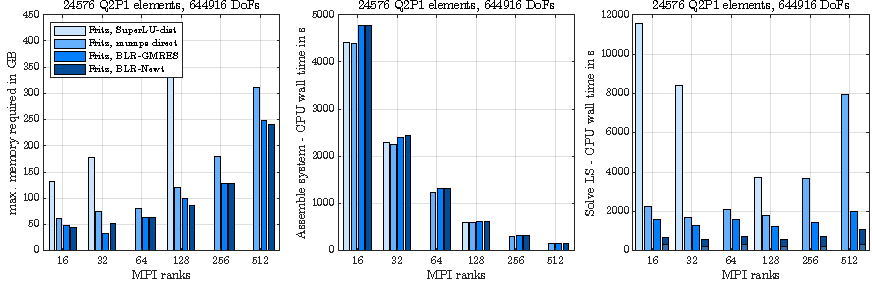
\includegraphics[width=\textwidth]{figures/FAU/figure_1.pdf}
  \caption{Comparison between four different solvers (SuperLU-dist, direct MUMPS, BLR-GMRES and BLR-Newt) applied to a medium size benchmark problem with 24676 elements and 644916 DoFs: memory usage (left), CPU wall time for system assembly (middle) and CPU wall to solve the linearized system (right).}
  \label{fig:four_solvers}
\end{figure}

The memory consumption (Figure \ref{fig:four_solvers}, left) is the clear bottleneck of the two direct solver variants -- even though the MUMPS direct solver performs significantly better. The memory consumption of the two iterative methods is comparable as we are using the same MUMPS-BLR preconditioner. The memory savings compared to the direct MUMPS solver can be attributed to the Block Low Rank factorization. As expected, system assembly scales perfectly (Figure \ref{fig:four_solvers}, middle). Figure \ref{fig:four_solvers}, right, shows the time spent in the linear solver. The direct MUMPS solver outperforms the direct SuperLU-dist solver but has scalability issues with significantly increasing CPU times for 256 and 512 MPI ranks (probably a side effect of the moderate system size). The BLR-GMRES combination is slightly faster than direct MUMPS and highlights that Block Low Rank factorization does not only save memory but also saves compute time. Finally, BLR-Newt provides the best performance so far. The Block Low Rank preconditioner is of sufficiently high quality to enable computations when it is computed only once at the beginning of each Newton iteration and reused in subsequent Newton--Raphson steps. Both BLR-GMRES and BLR-Newt show similar but less pronounced scalability issues as MUMPS direct.

Figure \ref{fig:full_brain_solvers} displays the influence of the MUMPS Block Low Rank factorization accuracy on the memory consumption (left), the time spent in the preconditioner (middle) and the time spent in the iterative GMRES solver (right). Here, we solved a more realistic problem that simulates a full brain indentation on a brain mesh reconstructed from MRI images. 

\begin{figure}[h]
  \centering
  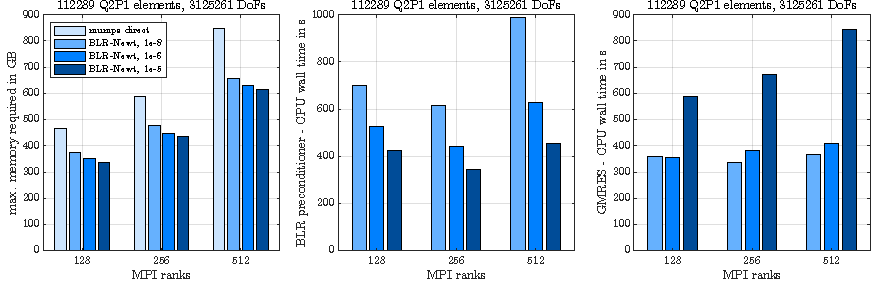
\includegraphics[width=\textwidth]{figures/FAU/figure_2.pdf}
  \caption{Influence of the BLR factorization accuracy for a coarse full brain indentation problem with 112289 elements and 3125261 DoFs: memory usage (left), CPU wall time for the MUMPS-BLR preconditioner (middle) and CPU wall time for the GMRES solver (right).}
  \label{fig:full_brain_solvers}
\end{figure}

As already indicated in Figure \ref{fig:four_solvers}, the BLR factorization reduces memory consumption as the the accuracy decreases. Of course, accuracy cannot be reduced indefinitely, but only as long as the preconditioner is still good enough for GMRES to converge (at all, or in a reasonable amount of iterations). For the more complex brain indentation we identified the accuracy limit at $\approx 10^{-5}$, while all previous benchmark problems could be performed with even lower accuracy of $\approx 10^{-4}$. Even though the total memory consumption increases with increasing number of MPI ranks, the maximum memory required per compute node decreases (from $\approx 180\,\mathrm{GB}$ on two, to $\approx 130\,\mathrm{GB}$ on four and $\approx 100\,\mathrm{GB}$ on eight compute nodes) -- a promising feature towards larges system sizes. As expected, reducing BLR accuracy also reduces the CPU time spent in the preconditioner. But, the accuracy of the BLR preconditioner also affects the performance of the subsequent GMRES solver. While performance is good up to an accuracy of $10^{-6}$, the number of GMRES iterations increases significantly for $10^{-5}$, outweighing the performance gains in the preconditioner. 

Performing a full brain indentation is already a great achievement and would not have been feasible at project start. Still, the currently highest mesh resolution that we can generate from MRI data is one refinement step further, i.e., eight times more elements and accordingly memory demanding. 

To provide proper region-dependent material parameters to our nonlinear poro-viscoelastic model, we need to ensure that our inverse parameter identification algorithm provides physically reasonable and unique parameter sets. Therefore, we reported on a numerical experiment in D2.2 that includes the lateral displacement into the inverse parameter identification. Our joint advances in computational efficiency of the ExaBrain repository allow us to extend the numerical study from poroelasticity to poro-viscoelasticity. Starting with a known set of poro-viscoelastic parameters, we performed a relaxation experiment of a cylindrical specimen and evaluated the total nominal stress as well as the lateral displacement. We then used this numerical “experimental” data as an input for our inverse parameter identification with 128 different sets
of initial parameters and included once only the total nominal stress into the objective function and once additionally the lateral displacement. Table \ref{tab:num_experiment} reports on the success rate (based on a normalized RMSE $<5\,\%$) of the modified inverse parameter identification. Clearly, using only the experimental measurement of the reaction force does not provide enough information to identify reliable parameter sets. In fact, only $12.5\,\%$ of the fits recovered the correct parameter set that was used to generate the numerical “experimental” data. The situation improves significantly including the lateral displacement -- a comparatively easy to obtain experimental measurement -- with $81.3\,\%$ correctly identified parameter sets. In addition $93.8\,\%$ of the fits provide physically reasonable results as they fit both, reaction force and lateral displacement. Using only the reaction force as an input, the success rate for fitting the lateral displacement drops to mere $15.6\,\%$.

\begin{table}[h]
    \centering
    \begin{tabular}{>{\centering\arraybackslash}m{3cm} >{\centering\arraybackslash}m{2.5cm} >{\centering\arraybackslash}m{2.5cm} >{\centering\arraybackslash}m{2cm} >{\centering\arraybackslash}m{3cm}}
    \toprule
         success rate &  fit reaction force & fit lateral displacement & fit both & recover correct parameter set\\ 
    \midrule
         only force & $96.9\,\%$ & $15.6\,\%$ & $15.6\,\%$ & $12.5\,\%$\\[10pt]
         force + lateral displacement & $94.5\,\%$ & $93.8\,\%$ & $93.8\,\%$ & $81.3\,\%$\\
    \bottomrule
    \end{tabular}
    \caption{Success rate (normalized RSME $<5\,\%$) of our poro-viscoelastic inverse parameter identification using once only the reaction force and once additionally the lateral displacement as an input. The results are based on 128 fits starting from different initial parameter sets.}
    \label{tab:num_experiment}
\end{table}

As a next step, we will use our new insights on the inverse parameter identification to identify brain region dependent poro-viscoelastic material parameters and apply them to test cases in full brain simulations.

\subsection{Liver (FVB-WIAS)}
This section reports on recent updates to the mixed-dimensional elasticity model and its application to liver simulation.

We finalized the coupling interface for connecting the developed three-dimen\-sio\-nal immersed mixed-dimension (3D-1D) elasticity model with an external solver for the simulation of one-dimensional hemodynamics. The method is based on a reduced Lagrangian multiplier method to consistently map the tissue pressure computed in the three-dimensional elasticity model into external one-dimensional pressures, as well as normal expansion or contraction of the vessels – computed within the 1D hemodynamics – into boundary conditions for the 3D elasticity solver.

The coupled scheme has been implemented building an interface to connect a high-order explicit finite volume scheme \citep{muller2016high} with the 3D reduced Lagrange multiplier elasticity solver (see Figure \ref{fig:coupling_scheme}). The two codes have independent discretizations and the 1D solver has an adaptive time-advancing scheme, which is independent from the time step used for the coupling.

\begin{figure}[h]
  \centering
  
\includegraphics[width=\textwidth]{figures/FVB-WIAS/figure_1.png}
  \caption{Schema of the coupling between the 3D reduced Lagrange multiplier and the 1D finite volume solvers.}
  \label{fig:coupling_scheme}
\end{figure}

The coupled model depends on the relation between three different discretizations: the 3D mesh for elasticity, the 1D discretization of vessel structures, and the discrete representation of the one-dimensional singular terms in the 3D model. We also integrated a recently developed preconditioner on the Augmented Lagrangian System \citep{benzi2026scalable}. The preconditioner allows a more efficient resolution of the saddle point problem, which, due to localization of the vascular structure, tends to be ill-conditioned. The coupled multi-scale model also marks the completion of milestone \#10 -- Multiscale Coupled Liver Model Completion.

Currently, we are performing detailed numerical tests to validate the model and the numerical method on a set of benchmark configurations, comparing stability, accuracy, and performance of different choices (see Figure \ref{fig:effect_refinement}).

\begin{figure}[h]
  \centering
  
\includegraphics[width=\textwidth]{figures/FVB-WIAS/figure_2.pdf}
  \caption{Effect of different longitudinal and transversal refinement of the 1D network in relation with the 3D mesh.}
  \label{fig:effect_refinement}
\end{figure}

The model will be used to perform a set of \emph{in silico} experiments to evaluate effective material behavior as a function of the time-dependent blood flow in the vascular network.

\begin{figure}[h]
  \centering
  
\includegraphics[width=0.4\textwidth]{figures/FVB-WIAS/figure_3.png}
  \caption{Discretized network from \citet{goirand2021network}, showing (white)  the points where singular forces are introduced in the elasticity model.}
  \label{fig:vessel_network}
\end{figure}

Ongoing work focuses also on the setup of a realistic computational model for the liver, considering a realistic three-dimensional mesh of the organ, and a vessel network (see Figure \ref{fig:vessel_network}) generated with constrained constructive optimization (CCO) \citep{kerautret2023opencco}.


\subsection{Mechanobiology (UNIBS)}

This section details recent advancements developed at the University of Brescia (UNIBS) regarding high-performance computational models for cell motility, implemented within the deal.II finite element library. Traditional continuum frameworks, such as the Larché–Cahn theory and classical Mixture Theories, often fail to capture the complex coupling of mechanical, chemical, and transport phenomena essential to cytoskeletal reorganization, particularly the dynamic assembly and disassembly of networks. A novel mathematical framework that extends \citet{salvadori2024generation} to incorporate these underlying kinematics and balance equations is forthcoming in \citet{salvadori2025chemo}.

Elucidating and controlling cell motility remains a fundamental scientific challenge, as it is the driving mechanism behind critical physiological and pathological processes, including tumor metastasis, embryogenesis, and hemostasis. These phenomena rely on force-bearing cytoskeletal networks that undergo continuous, dynamic assembly and disassembly in response to environmental cues. Central to this behavior is the complex interplay between actin cytoskeleton dynamics and receptor-mediated interactions at the interface of the cell membrane and the extracellular matrix. Our research framework is structured around two fundamental pillars:
\begin{enumerate}
    \item Actin Cytoskeleton Dynamics: Extending chemo-mechanical frameworks to include the interaction between actin transport, polymerization, and the mechanical forces driving membrane protrusion.
    \item Receptor-Ligand Interaction: Exploring how cell mechanics influence the che\-mo-diffusive behavior of adhesive receptors and their relocation on advecting lipid membranes.
\end{enumerate}
The Deliverable D2.2 detailed advancements concerning the first research pillar. This deliverable report provides critical insights into the space-time relocation of transmembrane proteins during cell motility. Characterizing this redistribution is essential for understanding how cells perceive environmental signals - specifically via chemotaxis (chemical gradients) and durotaxis (stiffness gradients) - and subsequently modulate their response to the extracellular matrix (ECM).

At this stage, we focus on the relocation of a receptor that is not primarily involved in cytoskeletal reorganization. Accordingly, the transport of this protein along the cell membrane does not influence the mechanical deformation of the cell bulk. This decoupling facilitates the use of a staggered algorithm that bypasses the need for prediction or correction phases. Specifically, at each time step, the mechanical problem in the bulk is solved first; once the updated geometric configuration is determined, the chemo-diffusive problem on the surface is solved subsequently, allowing for the use of independent time-discretization schemes \citep{martins2017new}.

The current implementation features significant numerical enhancements from \citet{serpelloni2023mechanobiology}, specifically through the integration of advanced stabilization methods and the transition to parallel distributed meshes and simulations. To suppress numerical oscillations, shock-capturing schemes introduce controlled artificial dissipation in the vicinity of steep gradients. This stabilization is locally adaptive: it provides high dissipation near shocks to maintain stability while remaining minimal in smooth regions to preserve solution accuracy.

The stabilization term is designed to be solution-dependent, utilizing the discrete residual as a shock sensor. In this framework, the residual within an element provides a local measure of how accurately the approximate solution satisfies the governing partial differential equation (PDE). In regions where the solution is smooth, the residual remains small, resulting in negligible artificial diffusivity. Conversely, near shocks or sharp gradients, the residual increases significantly, activating the localized diffusivity necessary to capture the solution in a non-oscillatory manner.

To leverage distributed-memory parallel computing, the implementation utilizes separate distributed triangulations for the bulk and the manifold. While the manifold mesh is extracted from the bulk boundary in another script, both are treated as independent objects within the current code. This decoupling allows for independent mesh operations; specifically, it should enable autonomous re-meshing of the manifold triangulation without affecting the bulk grid. Communication between these domains is managed by a dedicated transfer function that maps the displacement solution from the bulk to the manifold. Although the current framework supports this modularity, adaptive re-meshing of the manifold is reserved for future implementation.

\begin{figure}
  \centering
  
\includegraphics[width=0.9\textwidth]{figures/UNIBS/figure_1.png}
  \caption{3D simulation of an \emph{in-silico} cell during the initial stages of motility: the cell first undergoes adhesion to the $\mu$-slide substrate, followed by axisymmetrical spreading across the surface.}
  \label{fig:initial_motility}
\end{figure}

Our tests focused primarily on the transfer function of the displacement fields from the bulk to the manifold grid. At the best of our current tests and knowledge it seems to work well, as we can see from Figure \ref{fig:initial_motility}. However, we recognize that further investigations are required. Specifically, future work will focus on ensuring the robustness of the data mapping during autonomous re-meshing and optimizing the communication overhead in high-performance parallel environments. The following snapshots (see Figures \ref{fig:concentration_distribution}, \ref{fig:ligands_distribution} and \ref{fig:receptor_distribution}) illustrate the results of our simulations on the manifold. 

\begin{figure}
  \centering
  
\includegraphics[width=0.9\textwidth]{figures/UNIBS/figure_2.png}
  \caption{Concentration distribution in reference configuration and during adhesion phase.}
  \label{fig:concentration_distribution}
\end{figure}

\begin{figure}
  \centering
  
\includegraphics[width=0.9\textwidth]{figures/UNIBS/figure_3.png}
  \caption{Ligands distribution in reference configuration and during adhesion phase.}
  \label{fig:ligands_distribution}
\end{figure}

\begin{figure}
  \centering
  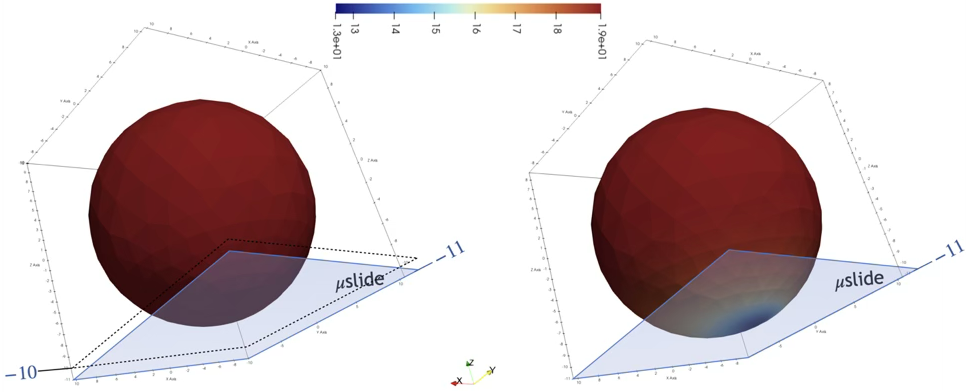
\includegraphics[width=0.9\textwidth]{figures/UNIBS/figure_4.png}
  \caption{Receptor distribution in reference configuration and during adhesion phase.}
  \label{fig:receptor_distribution}
\end{figure}

\subsection{Dualistic/eXact-Lab}
\subsubsection{Introduction}
First introduced in Deliverable D2.2, the PoC platform retains its three-component architecture (see Figure \ref{fig:PoC_architecture}), the deal.II-X Client, deal.II-X Cloud, and Coral execution engine, but each component has been substantially enhanced to support dispatching computational tasks to remote clusters while leveraging scheduling software such as Slurm.

\begin{figure}[h]
  \centering
  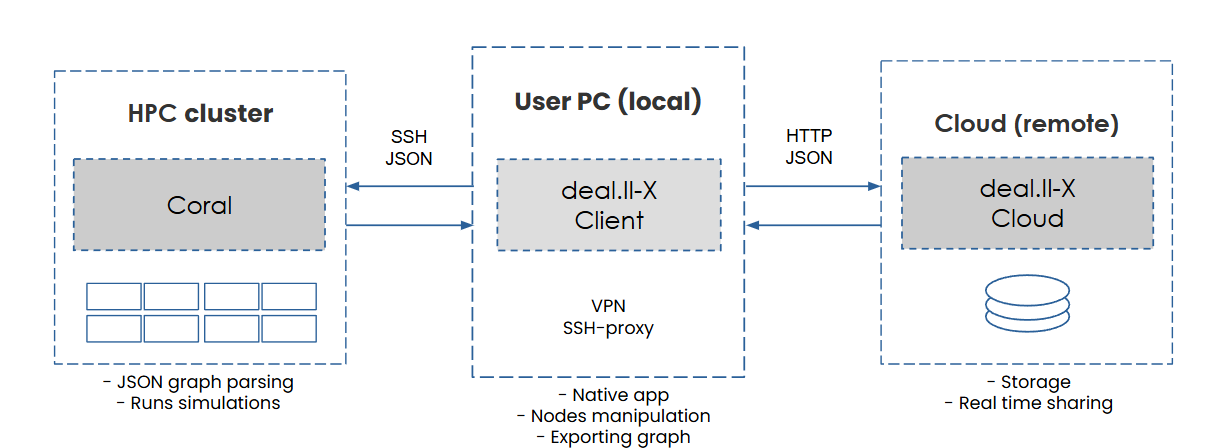
\includegraphics[width=\textwidth]{figures/Dualistic/figure_1.png}
  \caption{Three-component architecture of the PoC platform.}
  \label{fig:PoC_architecture}
\end{figure}

The three-component architecture from Section 2.6.2 of Deliverable D2.2 remains structurally unchanged: the Client acts as the central coordination point, the Cloud provides collaborative storage, and Coral executes computational graphs on target infrastructure. The approach outlined in Section 2.6.3 of Deliverable D2.2 has layered meta-scheduling capabilities across all three components, transforming the platform from a graphical workflow editor into a system for distributed computational task management. 

\subsubsection{Meta-Scheduling Capabilities}
The complete meta-scheduling workflow begins in the Client, where users construct computational graphs using the drag-and-drop interface introduced in Section 2.6.2 of Deliverable D2.2 (see Figure \ref{fig:graph_generation}). Once a graph is constructed and validated, the Client handles the entire task submission process through SSH-based communication with the target HPC cluster. The graph is exported as JSON conforming to Coral's network protocol, transferred via SFTP to the remote filesystem, and submitted to the Slurm scheduler. The Client maintains a persistent mapping between its internal job identifiers and the Slurm job IDs returned by the scheduler, storing this information using electron-store to ensure job tracking continues even if the application is closed and reopened. A polling system queries Slurm at regular intervals to retrieve job status, start times, and completion states, presenting this information through an expandable jobs panel that displays the history of submitted tasks.

A major enhancement for hierarchical task management comes in the form of network nodes, which represent encapsulated computational sub-graphs that can be created, saved, and reused as modular components within larger workflows. Network nodes allow users to decompose complex computational tasks into manageable units, with each network node containing its own internal graph of connected nodes. The meta-scheduler system introduces qualified IDs to uniquely identify nodes within this hierarchical structure. Network nodes are stored persistently in the Client's registry and can be dragged onto the canvas like any other node type.

\begin{figure}[h]
  \centering
  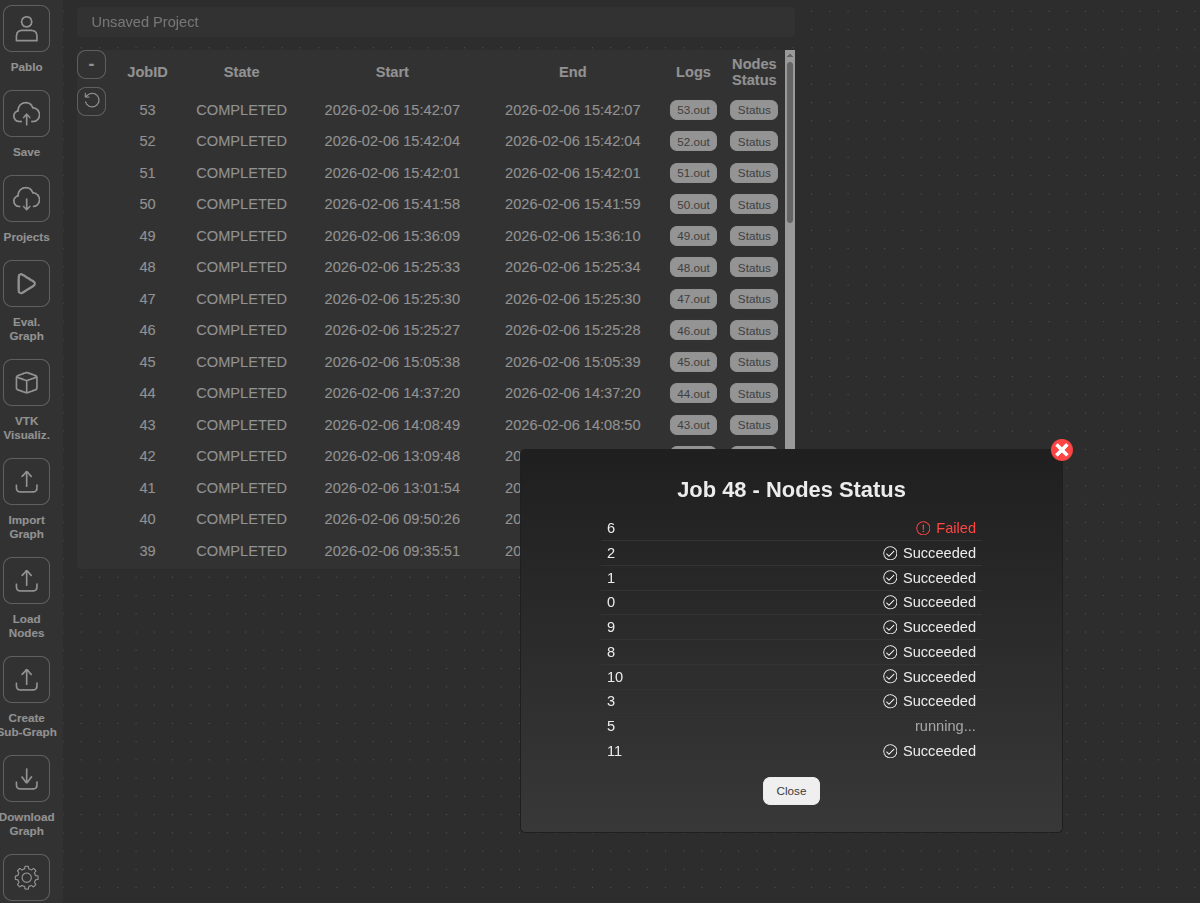
\includegraphics[width=0.9\textwidth]{figures/Dualistic/figure_2.png}
  \caption{Real-time visibility into the execution state of individual nodes within the graph.}
  \label{fig:individual_nodes}
\end{figure}

The execution status monitoring capabilities represent the most visible aspect of the meta-scheduler from a user perspective. When a computational task is running on a remote cluster, the Client provides real-time visibility into the execution state of individual nodes within the graph (see Figure \ref{fig:individual_nodes}). This is achieved through a filesystem-based status reporting mechanism implemented in Coral, where each node writes touch files to a designated directory. The Client queries this status directory via SSH to determine which nodes are currently running, which have completed, and which have failed. Users can open a modal dialog from the jobs panel to view a detailed breakdown of per-node execution status. The Client also provides access to the full Slurm output logs for each job, retrieving the .out files from the cluster and rendering them with specific colors depending on the type of the message.

Data persistence across sessions has been improved through the migration from browser localStorage to electron-store, which provides reliable storage in the Electron main process. The Client now persists the complete node registry, all user-defined network nodes, job history, and the mapping between internal and Slurm job IDs. Registry validation has been implemented to ensure that only nodes conforming to the expected protocol structure are made available in the sidebar, with abstract nodes and malformed entries automatically filtered out during import.

\begin{figure}[h]
  \centering
  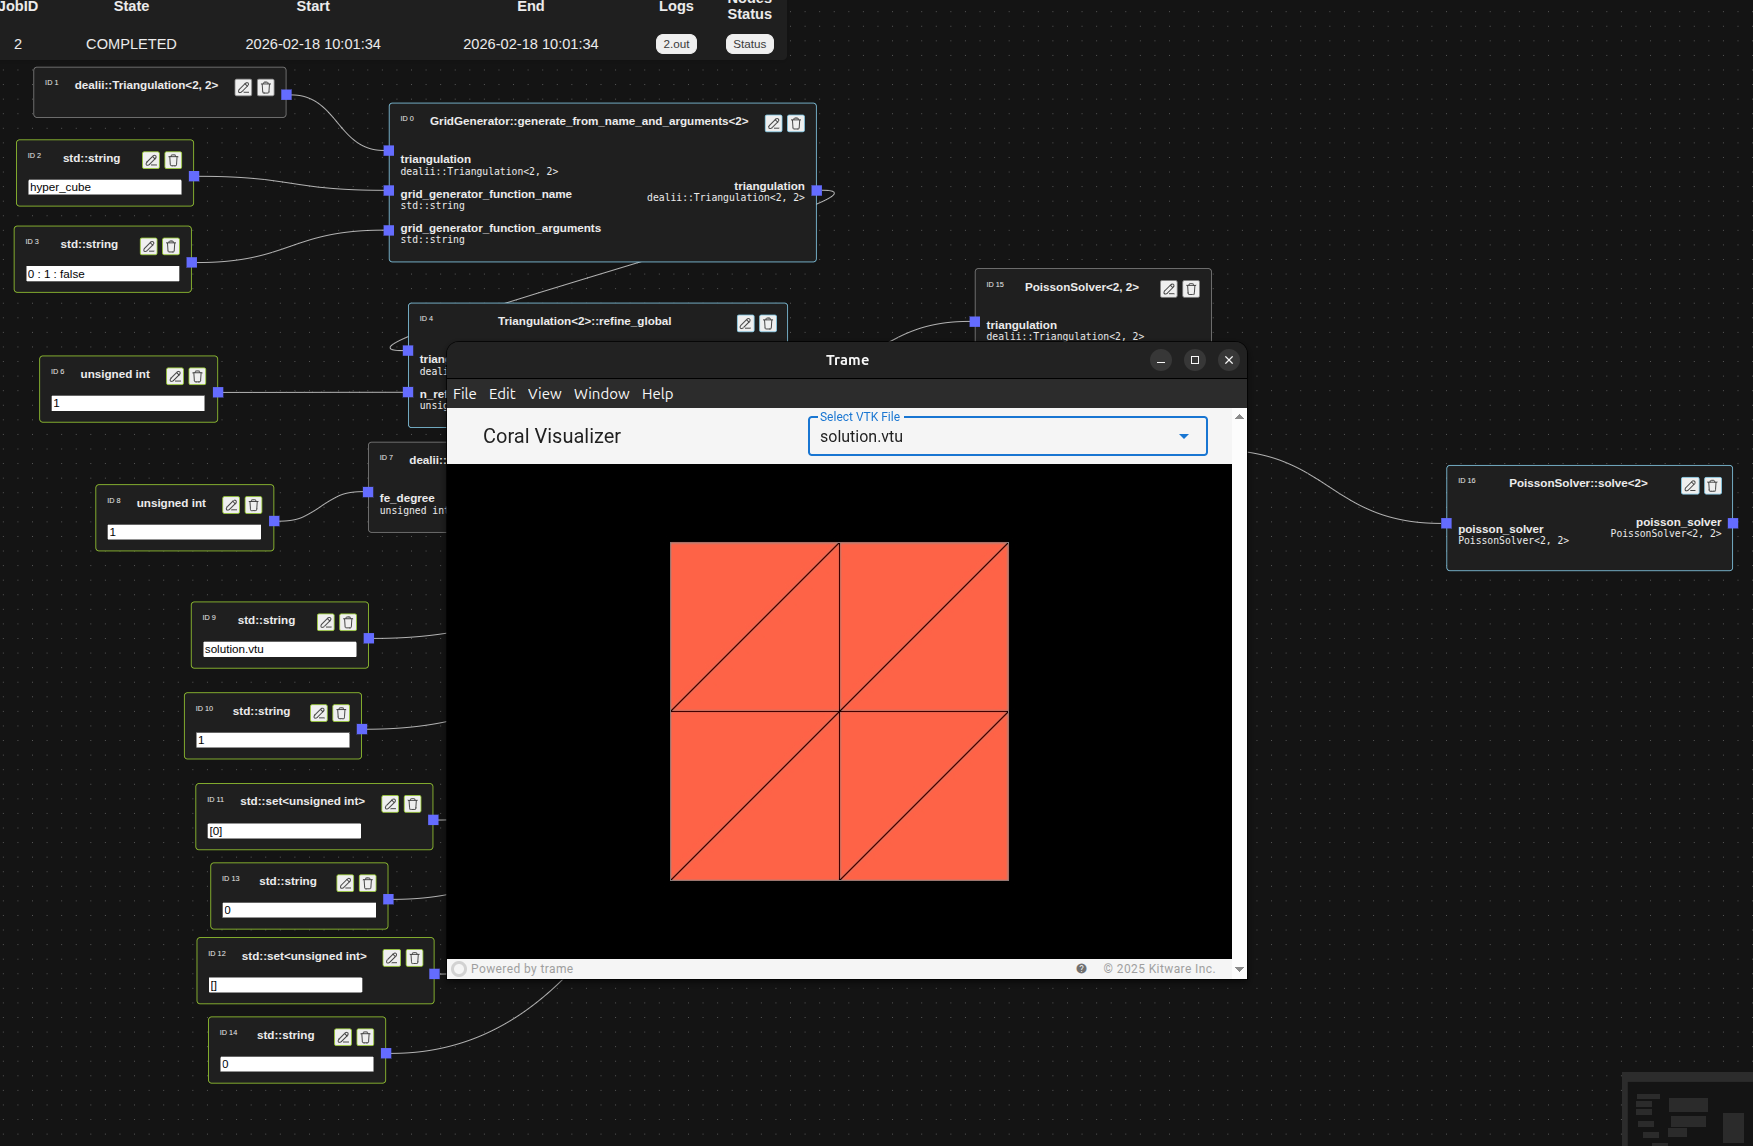
\includegraphics[width=0.9\textwidth]{figures/Dualistic/figure_3.png}
  \caption{An example of a graph that generates a 2D grid, with integrated visualization by means of Trame.}
  \label{fig:graph_generation}
\end{figure}

Taken together, the progress made in WP2.6 marks the completion of milestone
\#11 -- Deployment of the first version of the PoC WP2 platform.

\newpage

\section{{Conclusion}} \label{sec:conclusion}

In this document, we have reported the progress made in the digital twin applications of the deal.II-X project.

\bibliographystyle{plainnat}
\bibliography{../common/bibliography.bib}

\label{MyLastPage}

\end{document}